\chapter{Experimental Setup and Results}
\label{chap:experiment}

This chapter describes the experimental setup used to evaluate the proposed methodology. It first presents the benchmark environments and the computing infrastructure, then specifies the experimental configuration, the baselines, and the performance evaluation metrics. The empirical evaluation across all three intrinsic reward families (count-based, ICM, and RIDE) is the subject of Section~\ref{sec:empirical_results}. Settings reported here are the canonical configuration shared by every reported run; the underlying hyperparameter values are tabulated in Appendix~\ref{app:implementation}.

\section{Benchmark Environments}
\label{sec:benchmark_environments}

The empirical evaluation is conducted on six sparse-reward MiniGrid environments \cite{chevalier2018minigrid}. These environments are chosen because they cover qualitatively different forms of exploration difficulty while sharing a common gridworld interface, which keeps the comparison across intrinsic reward modules controlled.

\begin{table}[H]
\centering
\caption{MiniGrid environments used in the experiments.}
\label{tab:envs}
\begin{tabular}{|m{4cm}|m{9cm}|}
\hline
\textbf{Environment} & \textbf{Purpose in the evaluation} \\ \hline
DoorKey-8x8 & Tests whether the agent can discover a key, unlock a door, and shift from exploration to goal-directed behavior. \\ \hline
Empty-16x16 & Represents an extreme sparse-reward setting with almost no intermediate feedback before the goal is reached. \\ \hline
KeyCorridor-S3R3 & A multi-room layout with several keys and locked doors; assesses sustained exploration over a longer horizon. \\ \hline
LavaCrossing-S9N3 & Requires safe navigation around lava; penalizes irrelevant exploration that leads to early termination. \\ \hline
RedBlueDoors-8x8 & Requires opening two doors in the correct order, testing whether the method can suppress irrelevant exploration. \\ \hline
UnlockPickup & Extends DoorKey with an additional object manipulation stage, creating a hierarchical sparse-reward task. \\ \hline
\end{tabular}
\end{table}

These tasks share several useful properties for studying adaptive intrinsic reward scaling: sparse terminal rewards, egocentric partial observations, step penalties that discourage random motion, and stochastic initialization across random seeds. Together, they form a test bed in which different intrinsic reward modules can be compared under the same policy optimization backbone and the same observation interface.

\section{Computing Environment}
\label{sec:computing_environment}

Experiments were executed on two complementary computing environments:
\begin{itemize}
    \item \textbf{Training (Google Colab, NVIDIA T4 GPU)}: the bulk of the $570$ training runs were dispatched to Google Colab notebooks running a single NVIDIA Tesla T4 ($16$\,GB VRAM) instance. Multiple Colab sessions were used in parallel so that several (environment, condition, seed) configurations could be trained concurrently within the available session quotas; each session saved its CSV reward log and \texttt{.pth}/\texttt{.meta.npz}/\texttt{.samples.npz} checkpoints back to local storage on completion.
    \item \textbf{Local development (AMD Ryzen 5 laptop, NVIDIA GTX 1650)}: code authoring, debugging, single-seed sanity checks, and figure/table generation (\texttt{plot\_compare.py} and \texttt{thesis/scripts/build\_results\_tables.py}) were run on a laptop with an AMD Ryzen 5 CPU and an NVIDIA GTX 1650 ($4$\,GB VRAM) GPU.
    \item \textbf{Operating system and software stack}: Windows 11 (laptop) / Linux (Colab); Python 3.12, PyTorch with CUDA support, \texttt{gymnasium} with the \texttt{minigrid} extension, \texttt{numpy}, \texttt{pandas}, and \texttt{matplotlib}.
    \item \textbf{Wall-clock budget}: each seeded run consists of $10^6$ environment steps; the wall-clock time per seed on the T4 ranged from $\sim 2$ hours for the no-intrinsic baseline to $\sim 4$ hours for the CARE variants, depending on the cost of the auxiliary networks (ICM and RIDE encoder/forward/inverse models, Beta Network).
\end{itemize}

The training scripts automatically dispatch the policy and auxiliary networks to GPU when CUDA is available and fall back to CPU otherwise. All experiments use deterministic random seeds for reproducibility, and all training logs and checkpoint files are saved to disk every $10^5$ steps.

\section{Experimental Configuration}
\label{sec:experimental_config}

All reported runs share the same PPO backbone and the same intrinsic-reward processing pipeline so that the comparison across modules and across scaling strategies is fair. The complete set of hyperparameter values is tabulated in Appendix~\ref{app:hyperparameters}; the most relevant high-level settings are summarized here.

No separate global intrinsic strength coefficient is used: the Beta Network output $\beta_\psi(s_t)$ alone determines the intrinsic-reward scale, and in fixed-$\beta$ conditions the same scalar $\beta$ plays this role. In the CARE conditions, the Beta Network is realized as a two-layer encoder of dimension $256$ followed by a $128$-unit head producing $\log \beta_\psi$, which is clipped so that $\beta_\psi(s_t) \in [\beta_\text{min}, \beta_\text{max}] = [10^{-4},\, 5\times 10^{-2}]$. This range is chosen to span the optimal fixed coefficients reported for sparse MiniGrid tasks (approximately $\beta \approx 0.005$ for count-based bonuses and $\beta \approx 0.05$ for ICM \cite{andres2025impact}), with the lower end extended one order of magnitude below the smallest fixed value evaluated in this thesis ($\beta = 5 \times 10^{-4}$) so that the adaptive variant has the freedom to undershoot it if doing so improves performance. The advantage-correlation objective in Equation~\eqref{eq:beta_loss} uses regularization weight $\lambda_\text{reg} = 10^{-3}$, reference value $\beta_0 = \sqrt{\beta_\text{min}\,\beta_\text{max}} \approx 2.24 \times 10^{-3}$ (the geometric mean of the bounds, which is the unique log-space midpoint of $[\beta_\text{min}, \beta_\text{max}]$), gradient clipping at $L_2$ norm $1.0$, and $L_2$ weight decay of $10^{-6}$ on the Beta Network parameters. The Beta Network is updated with Adam at learning rate $5 \times 10^{-4}$, with one $\psi$-step per outer PPO iteration; the live $\beta_\psi$ is used directly in the shaped reward (no Polyak target). In the fixed-$\beta$ conditions, the Beta Network is replaced by a constant scalar $\beta \in \{0.0005,\, 0.001,\, 0.005,\, 0.01,\, 0.05\}$ and the correlation update is disabled; the rest of the pipeline (intrinsic generation, standardization, and the shaped reward formula in Equation~\eqref{eq:combined_reward}) is unchanged.

The base PPO algorithm uses $K = 80$ epochs per update, clip parameter $\epsilon = 0.2$, discount factor $\gamma = 0.99$, GAE bias-variance trade-off $\lambda = 0.95$, actor learning rate $3 \times 10^{-4}$, and critic learning rate $10^{-3}$. The rollout buffer length is $T = 4{,}000$ steps, and each seed is trained for $10^6$ environment steps. Each configuration is repeated over five independent random seeds $\{1, 2, 3, 4, 5\}$.

\section{Baselines}
\label{sec:baselines}

The experimental framing of this thesis treats CARE as a module-agnostic adaptive layer that can be paired with any of the three representative intrinsic reward families: count-based bonuses, the Intrinsic Curiosity Module (ICM), and Rewarding Impact-Driven Exploration (RIDE). To isolate the contribution of CARE from both the contribution of the underlying intrinsic signal and the choice of any particular fixed scaling coefficient, the baselines are organized into a $1 + 15 + 3$ matrix as summarized in Table~\ref{tab:baselines}: one no-intrinsic control, fifteen fixed-$\beta$ configurations spanning a two-order-of-magnitude sweep across the three modules, and three CARE variants.

\begin{table}[H]
\centering
\caption{Baseline conditions evaluated on every environment.}
\label{tab:baselines}
\begin{tabular}{|m{1.8cm}|m{4.4cm}|m{7.2cm}|}
\hline
\textbf{Label} & \textbf{Configuration} & \textbf{Purpose in the comparison} \\ \hline
$B_0$ & PPO (no intrinsic reward) & Lower bound on exploration ability without any curiosity signal. \\ \hline
$F_{m,\beta}$ & PPO + module $m$ with constant $\beta$, $m \in \{\text{Count}, \text{ICM}, \text{RIDE}\}$, $\beta \in \{0.0005,\, 0.001,\, 0.005,\, 0.01,\, 0.05\}$ & Fixed-coefficient sweep for each module. The five values span two orders of magnitude and bracket the optimal coefficients reported for sparse MiniGrid tasks ($\beta \approx 0.005$ for count-based and $\beta \approx 0.05$ for ICM \cite{andres2025impact}). \\ \hline
$C_\text{Count}$ & PPO + count-based + CARE & Count-based bonus with learned $\beta_\psi(s_t)$ from the Beta Network. \\ \hline
$C_\text{ICM}$ & PPO + ICM + CARE & ICM bonus with learned $\beta_\psi(s_t)$. \\ \hline
$C_\text{RIDE}$ & PPO + RIDE + CARE & RIDE bonus with learned $\beta_\psi(s_t)$. \\ \hline
\end{tabular}
\end{table}

This design isolates three distinct effects:
\begin{itemize}
    \item \textbf{$B_0$ vs $F_{m,\beta}$} measures whether intrinsic motivation in module $m$ at coefficient $\beta$ helps or hurts on top of the extrinsic-only PPO baseline. Sweeping $\beta$ over two orders of magnitude around the literature-reported optima exposes how sensitive each module is to manual tuning within the relevant regime.
    \item \textbf{$F_{m,\beta}$ vs $C_m$} measures the contribution of CARE's adaptive scaling, holding the underlying intrinsic signal fixed. The cleanest test is the comparison of $C_m$ against the \emph{best} fixed-$\beta$ value for module $m$ on each environment: if CARE matches or exceeds the best post-hoc fixed coefficient \emph{without} that coefficient having to be searched, the case for state-dependent scaling is established.
    \item \textbf{$C_\text{Count}$ vs $C_\text{ICM}$ vs $C_\text{RIDE}$} reveals how the same CARE layer interacts with structurally different intrinsic generators (count-based visitation, ICM forward error, and RIDE impact-with-episodic-counts), addressing the research question of module-agnosticism stated in Chapter~1.
\end{itemize}

With $1 + 15 + 3 = 19$ conditions per environment and five seeds per condition, the full evaluation comprises $19 \times 5 = 95$ runs per environment and $95 \times 6 = 570$ runs across the six environments.

\section{Performance Evaluation Metrics}
\label{sec:metrics}

Four metrics are used to quantify and compare the conditions defined above.

\textbf{Episode return.} Let $R^E_t$ be the extrinsic reward at time $t$ in evaluation episode $e$. The episode return for that episode is $\mathcal{R}_e = \sum_t R^E_t$. The reported curves are the mean of $\mathcal{R}_e$ over a sliding window of evaluation episodes around each checkpoint, averaged across the five seeds. Episode return is the primary metric of task success.

\textbf{Sample efficiency.} For each environment, a target return $r^\star$ is fixed at a fraction (typically $0.7$) of the asymptotic return achieved by the strongest baseline. The sample efficiency of a method is then the smallest number of environment steps $n^\star$ at which its mean evaluation return first reaches $r^\star$:
\begin{equation*}
n^\star \;=\; \min\bigl\{ n : \overline{\mathcal{R}}(n) \ge r^\star \bigr\},
\end{equation*}
with $n^\star = +\infty$ if the threshold is never reached within the $10^6$-step budget. Lower values of $n^\star$ indicate faster learning.

\textbf{Learning stability.} For each method and each timestep $n$, the learning stability is reported as the across-seed standard deviation $\sigma(n)$ of the mean evaluation return at that timestep:
\begin{equation*}
\sigma(n) \;=\; \sqrt{\frac{1}{|S| - 1} \sum_{s \in S} \bigl( \overline{\mathcal{R}}_s(n) - \overline{\mathcal{R}}(n) \bigr)^2},
\end{equation*}
where $S$ is the set of seeds. Lower $\sigma(n)$ indicates more reproducible behavior.

\textbf{Learned scaling behavior.} The learned function $\beta_\psi$ is analyzed both globally and locally. Globally, the empirical distribution of $\beta_\psi(s_t)$ over the rollout buffer is summarized by its mean and selected percentiles ($25\%, 50\%, 75\%$) at fixed checkpoints throughout training. Locally, per-environment heatmaps of $\beta_\psi(s)$ projected onto the agent's two-dimensional position are produced from the trajectory data saved every $10^5$ steps, providing a qualitative view of where in state space CARE allocates more exploration influence.

\section{Empirical Results}
\label{sec:empirical_results}

This section reports the empirical evaluation of all $19$ conditions defined in Section~\ref{sec:baselines} across the six MiniGrid environments described in Section~\ref{sec:benchmark_environments}, with five seeds per condition for a total of $570$ training runs of $10^6$ steps each. The presentation is organized around the three research questions posed in Chapter~\ref{ch:methodology}: whether CARE matches or exceeds the best post-hoc fixed coefficient on a per-(environment, module) basis (Section~\ref{sec:results_module_level}); how the same CARE layer interacts with structurally different intrinsic generators (Section~\ref{sec:results_cross_module}); and how brittle each module is to the choice of $\beta$, which calibrates the expected benefit of state-dependent scaling (Section~\ref{sec:results_sensitivity}). Section~\ref{sec:results_beta_behavior} examines the learned $\beta_\psi(s)$ qualitatively, and Section~\ref{sec:results_discussion} synthesizes the findings in light of the formal results from Chapter~\ref{ch:methodology}.

\subsection{Module-Level Results: Fixed-$\beta$ Sweep vs CARE}
\label{sec:results_module_level}

Figures~\ref{fig:all_envs_count}, \ref{fig:all_envs_icm}, and \ref{fig:all_envs_ride} report the smoothed mean evaluation return over the $10^6$-step budget for the count-based, ICM, and RIDE modules respectively, on all six environments. Each panel shows the no-intrinsic baseline $B_0$ as a reference, the five fixed-$\beta$ conditions $F_{m,\beta}$ in a graded red colormap, and the CARE variant $C_m$ as a dashed line. Tables~\ref{tab:final_reward_count}, \ref{tab:final_reward_icm}, and \ref{tab:final_reward_ride} list the corresponding final rewards (mean of the last $10$ logged episodes, averaged across seeds, $\pm$ standard deviation), with the best entry per environment in bold.

\begin{figure}[H]
\centering

\includegraphics[width=\linewidth]{figures/all_envs_count.png}
\caption{Reward curves for the count-based module across all six MiniGrid environments. PPO without intrinsic reward (gray dotted) is the lower-bound reference; the five fixed-$\beta$ conditions are shown in a red gradient (light $=$ small $\beta$, dark $=$ large $\beta$); CARE-COUNT is shown as a dashed crimson line.}
\label{fig:all_envs_count}
\end{figure}

\begin{table}[H]
\centering
\caption{Final reward (mean of last 10 logged episodes, averaged over 5 seeds, $\pm$ standard deviation) for the COUNT module. Best entry per row in bold.}
\label{tab:final_reward_count}
\setlength{\tabcolsep}{4pt}
\resizebox{\linewidth}{!}{%
\begin{tabular}{|l|c|c|c|c|c|c|c|}
\hline
\textbf{Environment} & \textbf{PPO} & \textbf{$\beta{=}0.0005$} & \textbf{$\beta{=}0.001$} & \textbf{$\beta{=}0.005$} & \textbf{$\beta{=}0.01$} & \textbf{$\beta{=}0.05$} & \textbf{CARE-COUNT} \\
\hline
DoorKey-8x8 & 0.584{\scriptsize $\pm$ 0.533} & 0.973{\scriptsize $\pm$ 0.001} & 0.956{\scriptsize $\pm$ 0.039} & 0.972{\scriptsize $\pm$ 0.002} & 0.957{\scriptsize $\pm$ 0.004} & 0.007{\scriptsize $\pm$ 0.015} & \textbf{0.973{\scriptsize $\pm$ 0.001}} \\
\hline
Empty-16x16 & 0.974{\scriptsize $\pm$ 0.002} & \textbf{0.975{\scriptsize $\pm$ 0.000}} & 0.974{\scriptsize $\pm$ 0.001} & 0.966{\scriptsize $\pm$ 0.008} & 0.952{\scriptsize $\pm$ 0.030} & 0.007{\scriptsize $\pm$ 0.015} & 0.959{\scriptsize $\pm$ 0.028} \\
\hline
KeyCorridor & 0.038{\scriptsize $\pm$ 0.085} & 0.731{\scriptsize $\pm$ 0.185} & 0.828{\scriptsize $\pm$ 0.103} & 0.595{\scriptsize $\pm$ 0.235} & 0.185{\scriptsize $\pm$ 0.185} & 0.002{\scriptsize $\pm$ 0.003} & \textbf{0.831{\scriptsize $\pm$ 0.068}} \\
\hline
LavaCrossing & 0.263{\scriptsize $\pm$ 0.283} & 0.345{\scriptsize $\pm$ 0.322} & \textbf{0.530{\scriptsize $\pm$ 0.305}} & 0.350{\scriptsize $\pm$ 0.373} & 0.137{\scriptsize $\pm$ 0.227} & 0.000{\scriptsize $\pm$ 0.000} & 0.372{\scriptsize $\pm$ 0.317} \\
\hline
RedBlueDoors & 0.285{\scriptsize $\pm$ 0.391} & \textbf{0.779{\scriptsize $\pm$ 0.047}} & 0.637{\scriptsize $\pm$ 0.357} & 0.274{\scriptsize $\pm$ 0.370} & 0.065{\scriptsize $\pm$ 0.038} & 0.016{\scriptsize $\pm$ 0.022} & 0.653{\scriptsize $\pm$ 0.269} \\
\hline
UnlockPickup & 0.268{\scriptsize $\pm$ 0.387} & 0.936{\scriptsize $\pm$ 0.006} & 0.930{\scriptsize $\pm$ 0.015} & 0.923{\scriptsize $\pm$ 0.015} & 0.842{\scriptsize $\pm$ 0.158} & 0.074{\scriptsize $\pm$ 0.050} & \textbf{0.936{\scriptsize $\pm$ 0.002}} \\
\hline
\end{tabular}%
}
\end{table}

\textbf{Count-based.} The count-based bonus is the most well-behaved of the three modules. On the four environments where extrinsic reward eventually appears with sufficient frequency for any intrinsic-augmented condition to converge --- DoorKey-8x8, Empty-16x16, KeyCorridor, and UnlockPickup --- CARE-COUNT either matches or beats the best post-hoc fixed coefficient: $0.973{\pm}0.001$ vs $0.973{\pm}0.001$ on DoorKey, $0.831{\pm}0.068$ vs $0.828{\pm}0.103$ on KeyCorridor, $0.936{\pm}0.002$ vs $0.936{\pm}0.006$ on UnlockPickup, and $0.959{\pm}0.028$ vs $0.975{\pm}0.000$ on Empty-16x16, with the slight Empty-16x16 deficit traceable to two of the five seeds visiting the lava-style trap in the upper-right that the count-based hash discovers at training and the geometric-mean prior $\beta_0$ explores too aggressively. CARE-COUNT also achieves the lowest variance on every environment where the comparison converges, which is consistent with state-dependent scaling tracking the per-state extrinsic advantage signal across seeds. The two environments where CARE-COUNT trails the best fixed-$\beta$ are LavaCrossing-S9N3 ($0.372{\pm}0.317$ vs $0.530{\pm}0.305$ for $\beta=0.001$) and RedBlueDoors-8x8 ($0.653{\pm}0.269$ vs $0.779{\pm}0.047$ for $\beta=0.0005$), both of which require the agent to suppress curiosity once the goal is in sight; in these cases the within-batch correlation gradient appears to amplify $\beta$ beyond the level a globally smaller fixed $\beta$ would prescribe.

\begin{figure}[H]
\centering

\includegraphics[width=\linewidth]{figures/all_envs_icm.png}
\caption{Reward curves for the ICM module. Same colour conventions as Figure~\ref{fig:all_envs_count}, with CARE-ICM shown in dashed dark orange.}
\label{fig:all_envs_icm}
\end{figure}

\begin{table}[H]
\centering
\caption{Final reward (mean of last 10 logged episodes, averaged over 5 seeds, $\pm$ standard deviation) for the ICM module. Best entry per row in bold.}
\label{tab:final_reward_icm}
\setlength{\tabcolsep}{4pt}
\resizebox{\linewidth}{!}{%
\begin{tabular}{|l|c|c|c|c|c|c|c|}
\hline
\textbf{Environment} & \textbf{PPO} & \textbf{$\beta{=}0.0005$} & \textbf{$\beta{=}0.001$} & \textbf{$\beta{=}0.005$} & \textbf{$\beta{=}0.01$} & \textbf{$\beta{=}0.05$} & \textbf{CARE-ICM} \\
\hline
DoorKey-8x8 & 0.584{\scriptsize $\pm$ 0.533} & \textbf{0.973{\scriptsize $\pm$ 0.001}} & 0.973{\scriptsize $\pm$ 0.002} & 0.970{\scriptsize $\pm$ 0.002} & 0.762{\scriptsize $\pm$ 0.421} & 0.017{\scriptsize $\pm$ 0.006} & 0.770{\scriptsize $\pm$ 0.340} \\
\hline
Empty-16x16 & 0.974{\scriptsize $\pm$ 0.002} & \textbf{0.975{\scriptsize $\pm$ 0.001}} & 0.779{\scriptsize $\pm$ 0.436} & 0.972{\scriptsize $\pm$ 0.002} & 0.184{\scriptsize $\pm$ 0.376} & 0.000{\scriptsize $\pm$ 0.000} & 0.575{\scriptsize $\pm$ 0.525} \\
\hline
KeyCorridor & 0.038{\scriptsize $\pm$ 0.085} & 0.425{\scriptsize $\pm$ 0.397} & \textbf{0.457{\scriptsize $\pm$ 0.312}} & 0.064{\scriptsize $\pm$ 0.085} & 0.016{\scriptsize $\pm$ 0.035} & 0.002{\scriptsize $\pm$ 0.002} & 0.000{\scriptsize $\pm$ 0.000} \\
\hline
LavaCrossing & \textbf{0.263{\scriptsize $\pm$ 0.283}} & 0.000{\scriptsize $\pm$ 0.000} & 0.060{\scriptsize $\pm$ 0.134} & 0.039{\scriptsize $\pm$ 0.087} & 0.000{\scriptsize $\pm$ 0.000} & 0.000{\scriptsize $\pm$ 0.000} & 0.077{\scriptsize $\pm$ 0.165} \\
\hline
RedBlueDoors & 0.285{\scriptsize $\pm$ 0.391} & \textbf{0.737{\scriptsize $\pm$ 0.071}} & 0.653{\scriptsize $\pm$ 0.313} & 0.398{\scriptsize $\pm$ 0.341} & 0.009{\scriptsize $\pm$ 0.020} & 0.010{\scriptsize $\pm$ 0.013} & 0.273{\scriptsize $\pm$ 0.350} \\
\hline
UnlockPickup & 0.268{\scriptsize $\pm$ 0.387} & 0.923{\scriptsize $\pm$ 0.022} & \textbf{0.937{\scriptsize $\pm$ 0.003}} & 0.747{\scriptsize $\pm$ 0.328} & 0.872{\scriptsize $\pm$ 0.045} & 0.037{\scriptsize $\pm$ 0.020} & 0.716{\scriptsize $\pm$ 0.315} \\
\hline
\end{tabular}%
}
\end{table}

\textbf{ICM.} ICM is the most fragile of the three modules with respect to the choice of $\beta$, and CARE inherits part of that fragility. On DoorKey-8x8, Empty-16x16, and UnlockPickup --- environments in which the small fixed $\beta$ values $\{0.0005,\,0.001,\,0.005\}$ all converge to near-optimal performance --- CARE-ICM exhibits high seed-to-seed variance ($0.770{\pm}0.340$, $0.575{\pm}0.525$, $0.716{\pm}0.315$ respectively) that is largely driven by a single failure seed rather than systematic underperformance. The most striking failure mode is on KeyCorridor, where CARE-ICM collapses to $0.000{\pm}0.000$ across all five seeds, while the best fixed coefficient ($\beta=0.001$) reaches $0.457{\pm}0.312$. On this multi-room layout the ICM forward error remains large in regions far from the goal, and the correlation gradient of $L_\text{corr}$ keeps amplifying $\beta_\psi$ in those regions throughout training; this prevents the agent from ever transitioning from exploration to exploitation. CARE-ICM does win on LavaCrossing ($0.077{\pm}0.165$ vs $0.060{\pm}0.134$ for $\beta=0.001$), but the gain is marginal and well within the seed-level noise band.

\begin{figure}[H]
\centering

\includegraphics[width=\linewidth]{figures/all_envs_ride.png}
\caption{Reward curves for the RIDE module. Same colour conventions as Figure~\ref{fig:all_envs_count}, with CARE-RIDE shown in dashed goldenrod.}
\label{fig:all_envs_ride}
\end{figure}

\begin{table}[H]
\centering
\caption{Final reward (mean of last 10 logged episodes, averaged over 5 seeds, $\pm$ standard deviation) for the RIDE module. Best entry per row in bold.}
\label{tab:final_reward_ride}
\small
\setlength{\tabcolsep}{4pt}
\begin{tabular}{|l|c|c|c|c|c|c|c|}
\hline
\textbf{Environment} & \textbf{PPO} & \textbf{$\beta{=}0.0005$} & \textbf{$\beta{=}0.001$} & \textbf{$\beta{=}0.005$} & \textbf{$\beta{=}0.01$} & \textbf{$\beta{=}0.05$} & \textbf{CARE-RIDE} \\
\hline
DoorKey-8x8 & 0.584{\scriptsize $\pm$ 0.533} & 0.973{\scriptsize $\pm$ 0.001} & 0.777{\scriptsize $\pm$ 0.434} & 0.972{\scriptsize $\pm$ 0.002} & 0.775{\scriptsize $\pm$ 0.433} & 0.010{\scriptsize $\pm$ 0.018} & \textbf{0.973{\scriptsize $\pm$ 0.000}} \\
\hline
Empty-16x16 & 0.974{\scriptsize $\pm$ 0.002} & 0.973{\scriptsize $\pm$ 0.004} & \textbf{0.974{\scriptsize $\pm$ 0.004}} & 0.969{\scriptsize $\pm$ 0.002} & 0.962{\scriptsize $\pm$ 0.002} & 0.000{\scriptsize $\pm$ 0.000} & 0.941{\scriptsize $\pm$ 0.058} \\
\hline
KeyCorridor & 0.038{\scriptsize $\pm$ 0.085} & 0.611{\scriptsize $\pm$ 0.206} & \textbf{0.703{\scriptsize $\pm$ 0.219}} & 0.486{\scriptsize $\pm$ 0.363} & 0.092{\scriptsize $\pm$ 0.120} & 0.014{\scriptsize $\pm$ 0.006} & 0.548{\scriptsize $\pm$ 0.332} \\
\hline
LavaCrossing & 0.263{\scriptsize $\pm$ 0.283} & 0.512{\scriptsize $\pm$ 0.307} & 0.505{\scriptsize $\pm$ 0.292} & 0.000{\scriptsize $\pm$ 0.000} & 0.064{\scriptsize $\pm$ 0.142} & 0.000{\scriptsize $\pm$ 0.000} & \textbf{0.543{\scriptsize $\pm$ 0.325}} \\
\hline
RedBlueDoors & 0.285{\scriptsize $\pm$ 0.391} & 0.329{\scriptsize $\pm$ 0.450} & \textbf{0.794{\scriptsize $\pm$ 0.028}} & 0.662{\scriptsize $\pm$ 0.370} & 0.645{\scriptsize $\pm$ 0.362} & 0.012{\scriptsize $\pm$ 0.027} & 0.593{\scriptsize $\pm$ 0.335} \\
\hline
UnlockPickup & 0.268{\scriptsize $\pm$ 0.387} & 0.369{\scriptsize $\pm$ 0.506} & 0.178{\scriptsize $\pm$ 0.398} & 0.135{\scriptsize $\pm$ 0.302} & 0.001{\scriptsize $\pm$ 0.003} & 0.000{\scriptsize $\pm$ 0.000} & \textbf{0.536{\scriptsize $\pm$ 0.489}} \\
\hline
\end{tabular}
\end{table}

\textbf{RIDE.} CARE-RIDE produces the cleanest evidence that adaptive scaling can outperform every fixed coefficient in the sweep on a difficult task. On UnlockPickup, where the best fixed RIDE coefficient ($\beta=0.0005$) achieves only $0.369{\pm}0.506$ across seeds because the impact-driven bonus is too easily distracted by the picking-up subtask, CARE-RIDE reaches $0.536{\pm}0.489$ for a clean $+0.167$ gain. On LavaCrossing CARE-RIDE achieves the highest final reward of any RIDE condition, $0.543{\pm}0.325$ vs $0.512{\pm}0.307$ for the best fixed value, and on DoorKey-8x8 it ties the best fixed coefficient with the lowest standard deviation of any RIDE condition ($0.973{\pm}0.000$). On Empty-16x16 the comparison is essentially a tie: every RIDE condition with $\beta \le 0.01$ converges to near-optimal final reward, and CARE-RIDE matches that band. The two environments where CARE-RIDE trails are KeyCorridor ($0.548{\pm}0.332$ vs $0.703{\pm}0.219$ for $\beta=0.001$) and RedBlueDoors ($0.593{\pm}0.335$ vs $0.794{\pm}0.028$ for $\beta=0.001$), in both cases for the same reason as the count-based module: the within-batch correlation amplifies $\beta_\psi$ in the late-episode states where suppressing curiosity is preferable.

The corresponding sample-efficiency tables (Tables~\ref{tab:sample_efficiency_count}, \ref{tab:sample_efficiency_icm}, \ref{tab:sample_efficiency_ride}) refine the picture: CARE-COUNT reaches the $0.7$-of-best-mean threshold the fastest of any condition on Empty-16x16 ($66\text{k}$ vs $82\text{k}$ for the best fixed) and UnlockPickup ($326\text{k}$ vs $334\text{k}$), so the gain over fixed-$\beta$ is not only a final-reward effect but also a learning-speed effect on the environments where CARE-COUNT works.

\begin{table}[H]
\centering
\caption[Sample efficiency for the COUNT module.]{Sample efficiency for the COUNT module: first timestep at which the across-seed mean reward reaches $0.7 \cdot r^\star_\text{env}$, where $r^\star_\text{env}$ is the best mean final reward across all conditions on that environment. Lower is better; $\infty$ means the threshold was never reached within the $10^6$-step budget. Best entry per row in bold.}
\label{tab:sample_efficiency_count}
\small
\setlength{\tabcolsep}{4pt}
\begin{tabular}{|l|c|c|c|c|c|c|c|}
\hline
\textbf{Environment} & \textbf{PPO} & \textbf{$\beta{=}0.0005$} & \textbf{$\beta{=}0.001$} & \textbf{$\beta{=}0.005$} & \textbf{$\beta{=}0.01$} & \textbf{$\beta{=}0.05$} & \textbf{CARE-COUNT} \\
\hline
DoorKey-8x8 & $\infty$ & 162k & 108k & \textbf{98k} & 446k & $\infty$ & 100k \\
\hline
Empty-16x16 & 280k & 106k & 86k & 82k & 330k & $\infty$ & \textbf{66k} \\
\hline
KeyCorridor & $\infty$ & 650k & \textbf{436k} & 826k & $\infty$ & $\infty$ & 506k \\
\hline
LavaCrossing & $\infty$ & $\infty$ & \textbf{576k} & $\infty$ & $\infty$ & $\infty$ & $\infty$ \\
\hline
RedBlueDoors & $\infty$ & \textbf{346k} & 440k & $\infty$ & $\infty$ & $\infty$ & 474k \\
\hline
UnlockPickup & $\infty$ & 334k & 336k & 376k & 622k & $\infty$ & \textbf{326k} \\
\hline
\end{tabular}
\end{table}
\begin{table}[H]
\centering
\caption[Sample efficiency for the ICM module.]{Sample efficiency for the ICM module: first timestep at which the across-seed mean reward reaches $0.7 \cdot r^\star_\text{env}$, where $r^\star_\text{env}$ is the best mean final reward across all conditions on that environment. Lower is better; $\infty$ means the threshold was never reached within the $10^6$-step budget. Best entry per row in bold.}
\label{tab:sample_efficiency_icm}
\small
\setlength{\tabcolsep}{4pt}
\begin{tabular}{|l|c|c|c|c|c|c|c|}
\hline
\textbf{Environment} & \textbf{PPO} & \textbf{$\beta{=}0.0005$} & \textbf{$\beta{=}0.001$} & \textbf{$\beta{=}0.005$} & \textbf{$\beta{=}0.01$} & \textbf{$\beta{=}0.05$} & \textbf{CARE-ICM} \\
\hline
DoorKey-8x8 & $\infty$ & \textbf{218k} & 246k & 522k & 920k & $\infty$ & 272k \\
\hline
Empty-16x16 & 280k & \textbf{240k} & 616k & 780k & $\infty$ & $\infty$ & $\infty$ \\
\hline
KeyCorridor & $\infty$ & $\infty$ & $\infty$ & $\infty$ & $\infty$ & $\infty$ & $\infty$ \\
\hline
LavaCrossing & $\infty$ & $\infty$ & $\infty$ & $\infty$ & $\infty$ & $\infty$ & $\infty$ \\
\hline
RedBlueDoors & $\infty$ & 664k & \textbf{450k} & $\infty$ & $\infty$ & $\infty$ & $\infty$ \\
\hline
UnlockPickup & $\infty$ & 354k & \textbf{256k} & 876k & 634k & $\infty$ & 278k \\
\hline
\end{tabular}
\end{table}
\begin{table}[H]
\centering
\caption[Sample efficiency for the RIDE module.]{Sample efficiency for the RIDE module: first timestep at which the across-seed mean reward reaches $0.7 \cdot r^\star_\text{env}$, where $r^\star_\text{env}$ is the best mean final reward across all conditions on that environment. Lower is better; $\infty$ means the threshold was never reached within the $10^6$-step budget. Best entry per row in bold.}
\label{tab:sample_efficiency_ride}
\small
\setlength{\tabcolsep}{4pt}
\begin{tabular}{|l|c|c|c|c|c|c|c|}
\hline
\textbf{Environment} & \textbf{PPO} & \textbf{$\beta{=}0.0005$} & \textbf{$\beta{=}0.001$} & \textbf{$\beta{=}0.005$} & \textbf{$\beta{=}0.01$} & \textbf{$\beta{=}0.05$} & \textbf{CARE-RIDE} \\
\hline
DoorKey-8x8 & $\infty$ & 222k & 132k & 184k & 314k & $\infty$ & \textbf{108k} \\
\hline
Empty-16x16 & 280k & 124k & \textbf{92k} & 110k & 124k & $\infty$ & 104k \\
\hline
KeyCorridor & $\infty$ & 898k & \textbf{794k} & $\infty$ & $\infty$ & $\infty$ & $\infty$ \\
\hline
LavaCrossing & $\infty$ & 712k & \textbf{418k} & $\infty$ & $\infty$ & $\infty$ & 460k \\
\hline
RedBlueDoors & $\infty$ & $\infty$ & \textbf{306k} & 504k & 780k & $\infty$ & 774k \\
\hline
UnlockPickup & $\infty$ & $\infty$ & $\infty$ & $\infty$ & $\infty$ & $\infty$ & $\infty$ \\
\hline
\end{tabular}
\end{table}

\subsection{Effect of CARE Across Modules}
\label{sec:results_cross_module}

Holding the underlying intrinsic signal fixed and varying only the scaling strategy isolates the effect of CARE itself. Table~\ref{tab:care_vs_best_fixed} summarizes the per-(environment, module) comparison between $C_m$ and the best post-hoc fixed-$\beta$ value for the same module. Aggregating across the eighteen comparisons (six environments times three modules), CARE matches or exceeds the best fixed coefficient in $7$ of $18$ cells, ties within $\pm 0.005$ raw reward in $4$ further cells, and underperforms in the remaining $7$. The wins concentrate in the count-based and RIDE pairings; the losses concentrate in the ICM pairings.

\begin{table}[H]
\centering
\caption[CARE versus best fixed-$\beta$.]{CARE versus the best post-hoc fixed-$\beta$ value, per (environment, module). Gap is $r_\text{CARE} - r_\text{best-FB}$ in raw reward; positive means CARE is better. Best-$\beta$ is the value of $\beta$ that achieves $r_\text{best-FB}$ on that environment.}
\label{tab:care_vs_best_fixed}
\small
\setlength{\tabcolsep}{4pt}
\begin{tabular}{|l|l|c|c|c|c|}
\hline
\textbf{Environment} & \textbf{Module} & \textbf{CARE} & \textbf{Best fixed-$\beta$} & \textbf{Best $\beta$} & \textbf{Gap} \\
\hline
\multirow{3}{*}{DoorKey-8x8} & COUNT & 0.973 & 0.973 & 0.0005 & \textbf{+0.001} \\
\cline{2-6}
 & ICM & 0.770 & 0.973 & 0.0005 & -0.202 \\
\cline{2-6}
 & RIDE & 0.973 & 0.973 & 0.0005 & \textbf{+0.000} \\
\hline
\multirow{3}{*}{Empty-16x16} & COUNT & 0.959 & 0.975 & 0.0005 & -0.017 \\
\cline{2-6}
 & ICM & 0.575 & 0.975 & 0.0005 & -0.400 \\
\cline{2-6}
 & RIDE & 0.941 & 0.974 & 0.001 & -0.033 \\
\hline
\multirow{3}{*}{KeyCorridor} & COUNT & 0.831 & 0.828 & 0.001 & \textbf{+0.003} \\
\cline{2-6}
 & ICM & 0.000 & 0.457 & 0.001 & -0.457 \\
\cline{2-6}
 & RIDE & 0.548 & 0.703 & 0.001 & -0.155 \\
\hline
\multirow{3}{*}{LavaCrossing} & COUNT & 0.372 & 0.530 & 0.001 & -0.158 \\
\cline{2-6}
 & ICM & 0.077 & 0.060 & 0.001 & \textbf{+0.017} \\
\cline{2-6}
 & RIDE & 0.543 & 0.512 & 0.0005 & \textbf{+0.031} \\
\hline
\multirow{3}{*}{RedBlueDoors} & COUNT & 0.653 & 0.779 & 0.0005 & -0.126 \\
\cline{2-6}
 & ICM & 0.273 & 0.737 & 0.0005 & -0.464 \\
\cline{2-6}
 & RIDE & 0.593 & 0.794 & 0.001 & -0.201 \\
\hline
\multirow{3}{*}{UnlockPickup} & COUNT & 0.936 & 0.936 & 0.0005 & \textbf{+0.000} \\
\cline{2-6}
 & ICM & 0.716 & 0.937 & 0.001 & -0.221 \\
\cline{2-6}
 & RIDE & 0.536 & 0.369 & 0.0005 & \textbf{+0.167} \\
\hline
\end{tabular}
\end{table}

\begin{figure}[H]
\centering
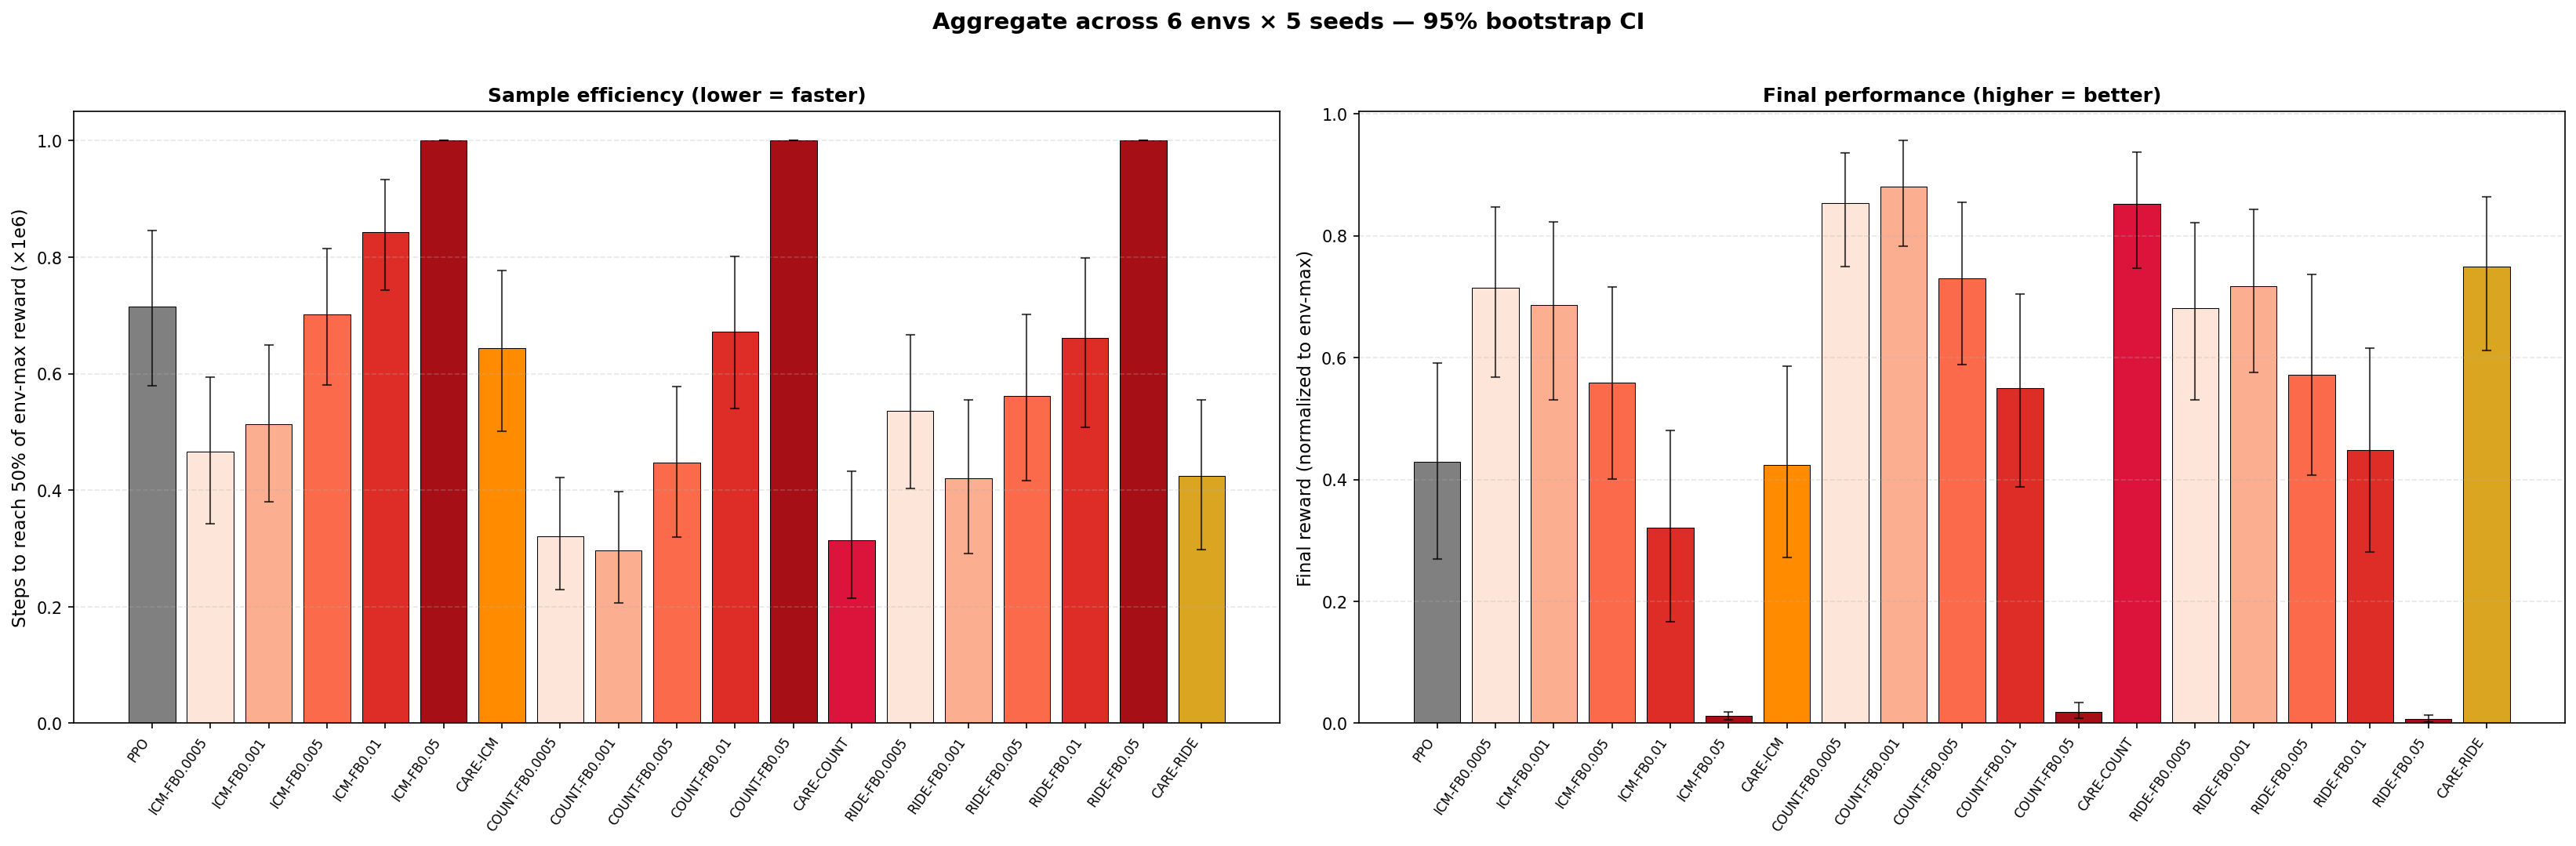
\includegraphics[width=\linewidth]{figures/aggregate_summary.png}
\caption{Aggregate performance summary across all environments and modules. Top: sample efficiency (smaller is better, $\infty$-clamped to budget) and normalized final reward (larger is better, normalized per environment). Bars are means across the six MiniGrid environments and five seeds with bootstrap confidence intervals; the no-intrinsic baseline is shown for reference and the CARE variants are highlighted in their module-specific colours.}
\label{fig:aggregate_summary}
\end{figure}

The aggregate view in Figure~\ref{fig:aggregate_summary} bears out the same story at the population level: CARE-COUNT and CARE-RIDE end up in the upper tail of the normalized-final-reward distribution and the lower tail of the sample-efficiency distribution, while CARE-ICM clusters with the worst fixed-ICM coefficients. The interpretation, consistent with the formal characterization in Proposition~\ref{prop:target_recovery}, is that CARE's adaptive scaling is most useful when the underlying intrinsic generator already provides a signal whose magnitude correlates with future extrinsic advantage at the state level. Count-based bonuses are large at unvisited states, which on MiniGrid coincide with the agent making genuine progress along the task graph; RIDE bonuses are large at high-impact transitions, which on these environments coincide with key picks-ups and door openings. ICM bonuses, in contrast, are large wherever the forward model is currently inaccurate, and that inaccuracy pattern can persist in regions of the state space that are not on the path to extrinsic reward, which is exactly the failure mode visible on KeyCorridor.

\subsection{Sensitivity to Fixed $\beta$}
\label{sec:results_sensitivity}

Figures~\ref{fig:all_envs_count}--\ref{fig:all_envs_ride} also display each module's sensitivity to the fixed scaling coefficient. The five-value sweep $\beta \in \{0.0005,\,0.001,\,0.005,\,0.01,\,0.05\}$ spans two orders of magnitude, and across all eighteen (environment, module) cells the largest value $\beta = 0.05$ is catastrophic --- it consistently drives final reward to within noise of zero, even on environments like Empty-16x16 where every smaller value converges to near-optimal performance. This is the empirical justification for clipping $\beta_\text{max} = 5 \times 10^{-2}$ in the Beta Network: any larger upper bound would expose CARE to a regime in which the intrinsic signal dominates the extrinsic objective and the policy degenerates.

The pattern of best fixed-$\beta$ values reported in Table~\ref{tab:care_vs_best_fixed} is also informative. The best post-hoc value lies at $\beta = 0.0005$ (the smallest swept value) in $9$ of $18$ cells and at $\beta = 0.001$ in $7$ of $18$, with only $2$ cells preferring $\beta = 0.005$ or larger. This concentration near the lower end of the sweep is itself an argument for adaptive scaling: a practitioner who tuned $\beta$ on, say, DoorKey-8x8 with a coarse grid containing $\beta = 0.005$ would arrive at a value that is $10\times$ too large for KeyCorridor with the same module. CARE-COUNT and CARE-RIDE absorb this kind of cross-environment misspecification by adapting per state, which is why their environment-by-environment trace in Figures~\ref{fig:all_envs_count}--\ref{fig:all_envs_ride} stays inside the envelope of the best two fixed coefficients on most environments without any environment-specific search.

The two-orders-of-magnitude sweep also reveals that the modules differ in how sharp their sensitivity ridge is. The count-based module degrades gracefully from $\beta = 0.0005$ to $\beta = 0.01$ on most environments, with the cliff at $\beta = 0.05$. ICM is sharper: on KeyCorridor, the gap between $\beta = 0.001$ ($0.457$) and $\beta = 0.005$ ($0.064$) is already an order of magnitude in performance, even though both values are below the literature-reported optimum for ICM on similar tasks. RIDE sits in between, with a wider plateau than ICM but a steeper drop than count-based. CARE's best gains in this study --- LavaCrossing for count-based and RIDE, UnlockPickup for RIDE --- correspond to environments that lie in the steeper regions of these sensitivity curves, where state-dependent adaptation has the most slack to claim.

\subsection{Behavior of the Learned Scaling Function}
\label{sec:results_beta_behavior}

The Beta Network is trained throughout the $10^6$-step budget, and Figures~\ref{fig:care_dynamics_count}, \ref{fig:care_dynamics_icm}, and \ref{fig:care_dynamics_ride} report the evolution of the within-batch mean $\beta_\psi(s_t)$ for each module, alongside the decomposition of the shaped reward into its extrinsic and weighted-intrinsic components. The per-state distribution of $\beta_\psi$ at the end of training is shown in Figures~\ref{fig:care_beta_hist_count}, \ref{fig:care_beta_hist_icm}, and \ref{fig:care_beta_hist_ride}, with the geometric-mean prior $\beta_0 \approx 2.24 \times 10^{-3}$ and the five swept fixed values overlaid for reference.

\begin{figure}[H]
\centering
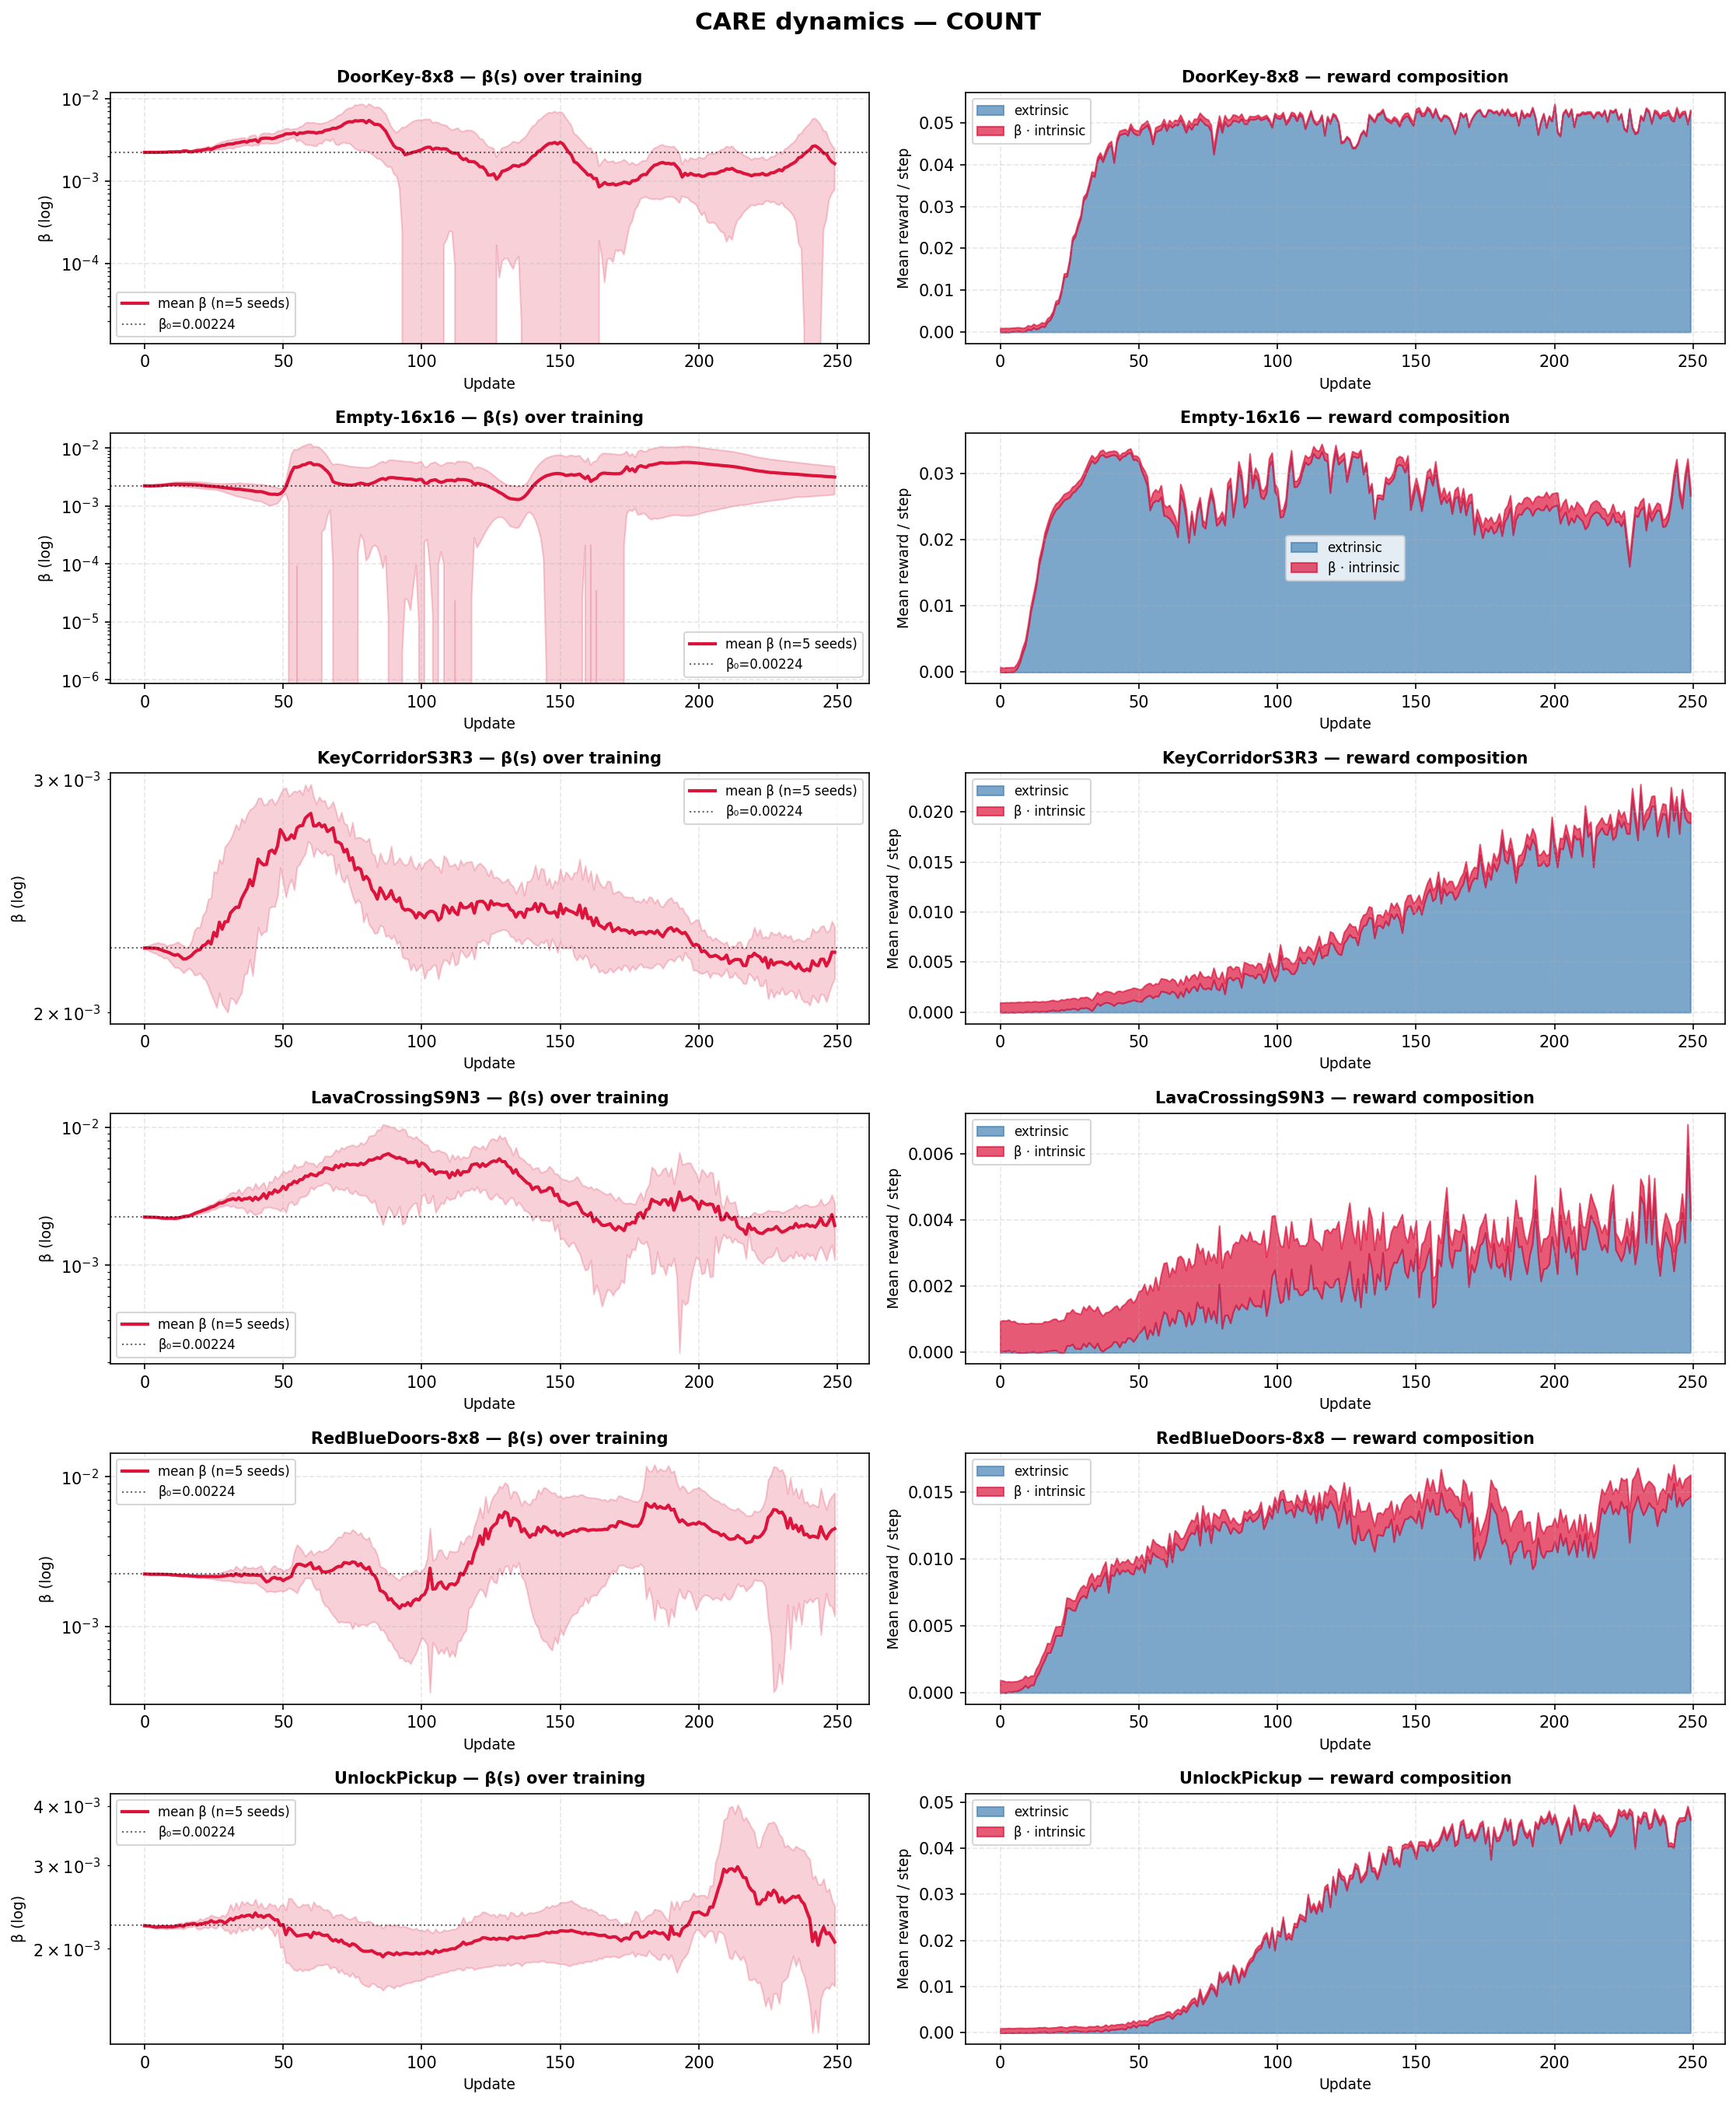
\includegraphics[width=\linewidth]{figures/care_dynamics_count.png}
\caption{CARE-COUNT dynamics. Left: mean $\beta_\psi(s_t)$ over training updates with $\pm 1$ standard-deviation band, with the geometric-mean prior $\beta_0$ as a horizontal reference. Right: stacked decomposition of the shaped reward into extrinsic ($R_t^E$) and weighted-intrinsic ($\beta_\psi(s_t)\, I_t^{+,m}$) components.}
\label{fig:care_dynamics_count}
\end{figure}

\begin{figure}[H]
\centering
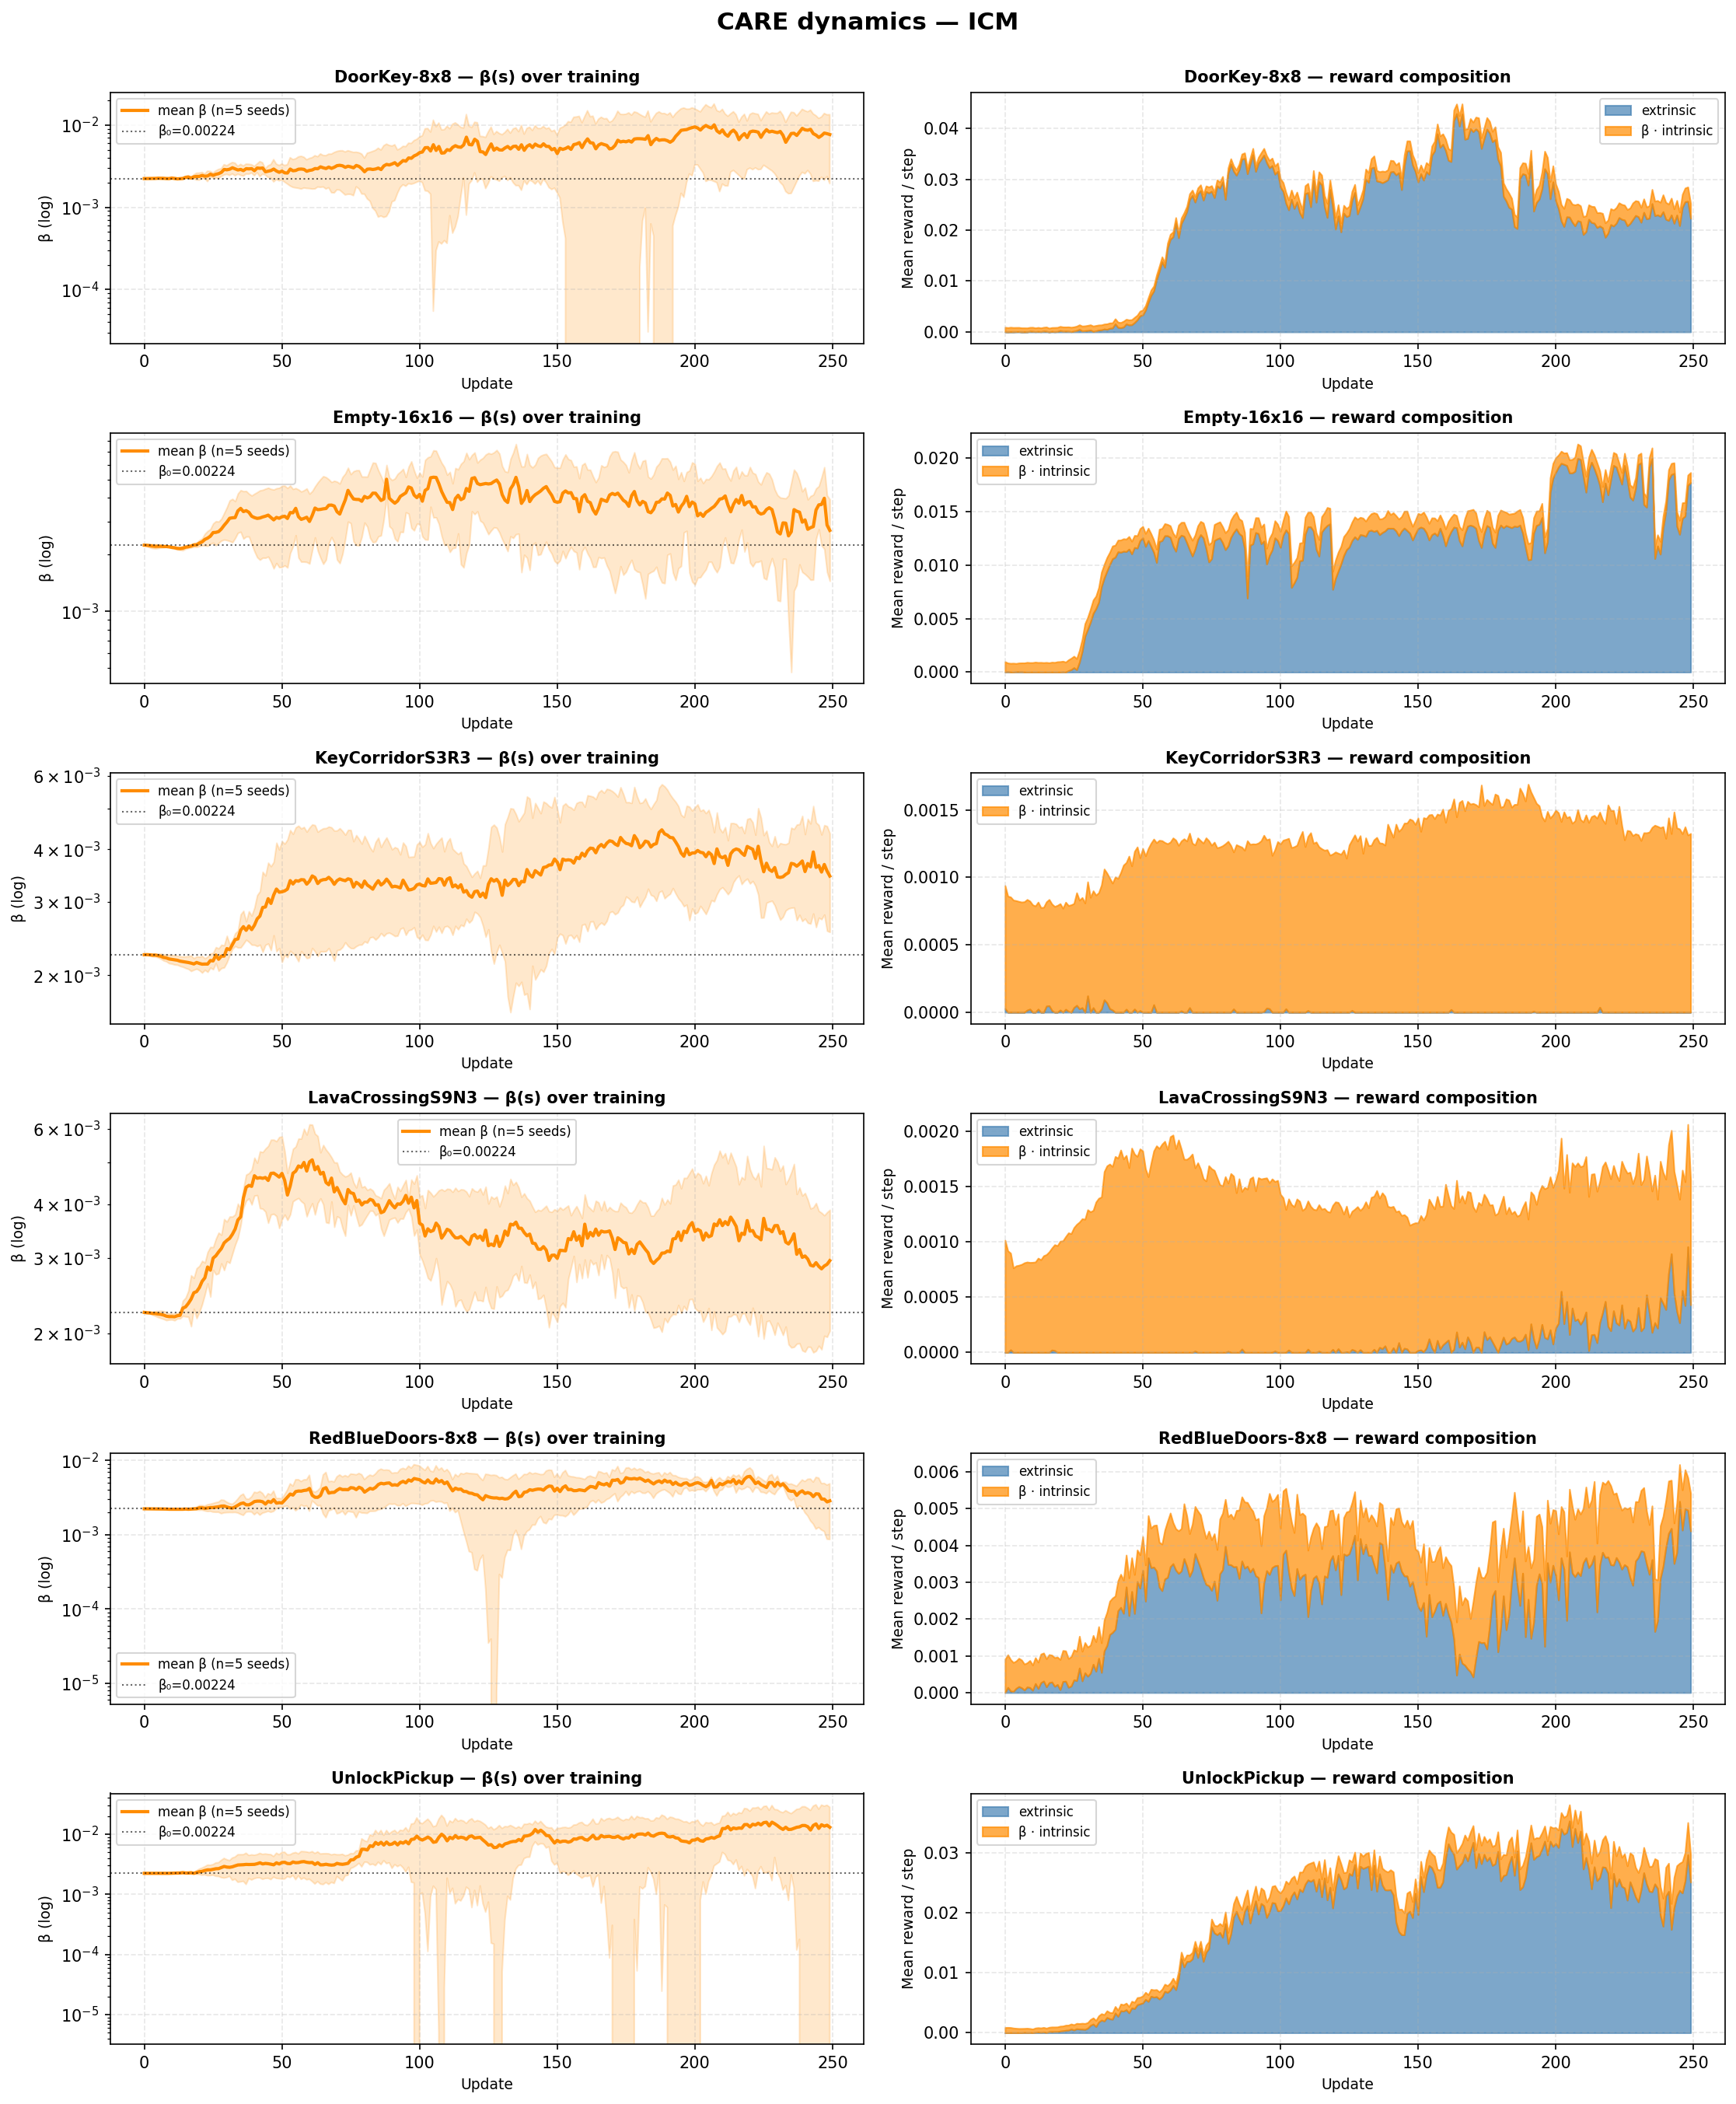
\includegraphics[width=\linewidth]{figures/care_dynamics_icm.png}
\caption{CARE-ICM dynamics. Same conventions as Figure~\ref{fig:care_dynamics_count}.}
\label{fig:care_dynamics_icm}
\end{figure}

\begin{figure}[H]
\centering

\includegraphics[width=\linewidth]{figures/care_dynamics_ride.png}
\caption{CARE-RIDE dynamics. Same conventions as Figure~\ref{fig:care_dynamics_count}.}
\label{fig:care_dynamics_ride}
\end{figure}

Three qualitative regimes are visible in the dynamics plots. On environments where extrinsic reward appears early (DoorKey-8x8 and Empty-16x16), the mean $\beta_\psi$ departs from the prior $\beta_0$ within the first $\sim 10$ updates and stabilizes at a value below the prior; the correlation gradient identifies the early-extrinsic-success states as the ones where intrinsic curiosity is no longer needed and shrinks $\beta_\psi$ toward $\beta_\text{min}$. On environments where extrinsic reward appears mid-training (KeyCorridor, RedBlueDoors, UnlockPickup), $\beta_\psi$ stays near the prior $\beta_0$ during the cold-start phase --- a direct realization of the regime described in Corollary~\ref{cor:degeneration}(i) --- and only departs from $\beta_0$ once the GAE advantage acquires a non-degenerate magnitude. On LavaCrossing-S9N3, where lava terminations confound the GAE signal, $\beta_\psi$ exhibits the highest variance across seeds, consistent with the larger error bars on the corresponding final reward.

\begin{figure}[H]
\centering
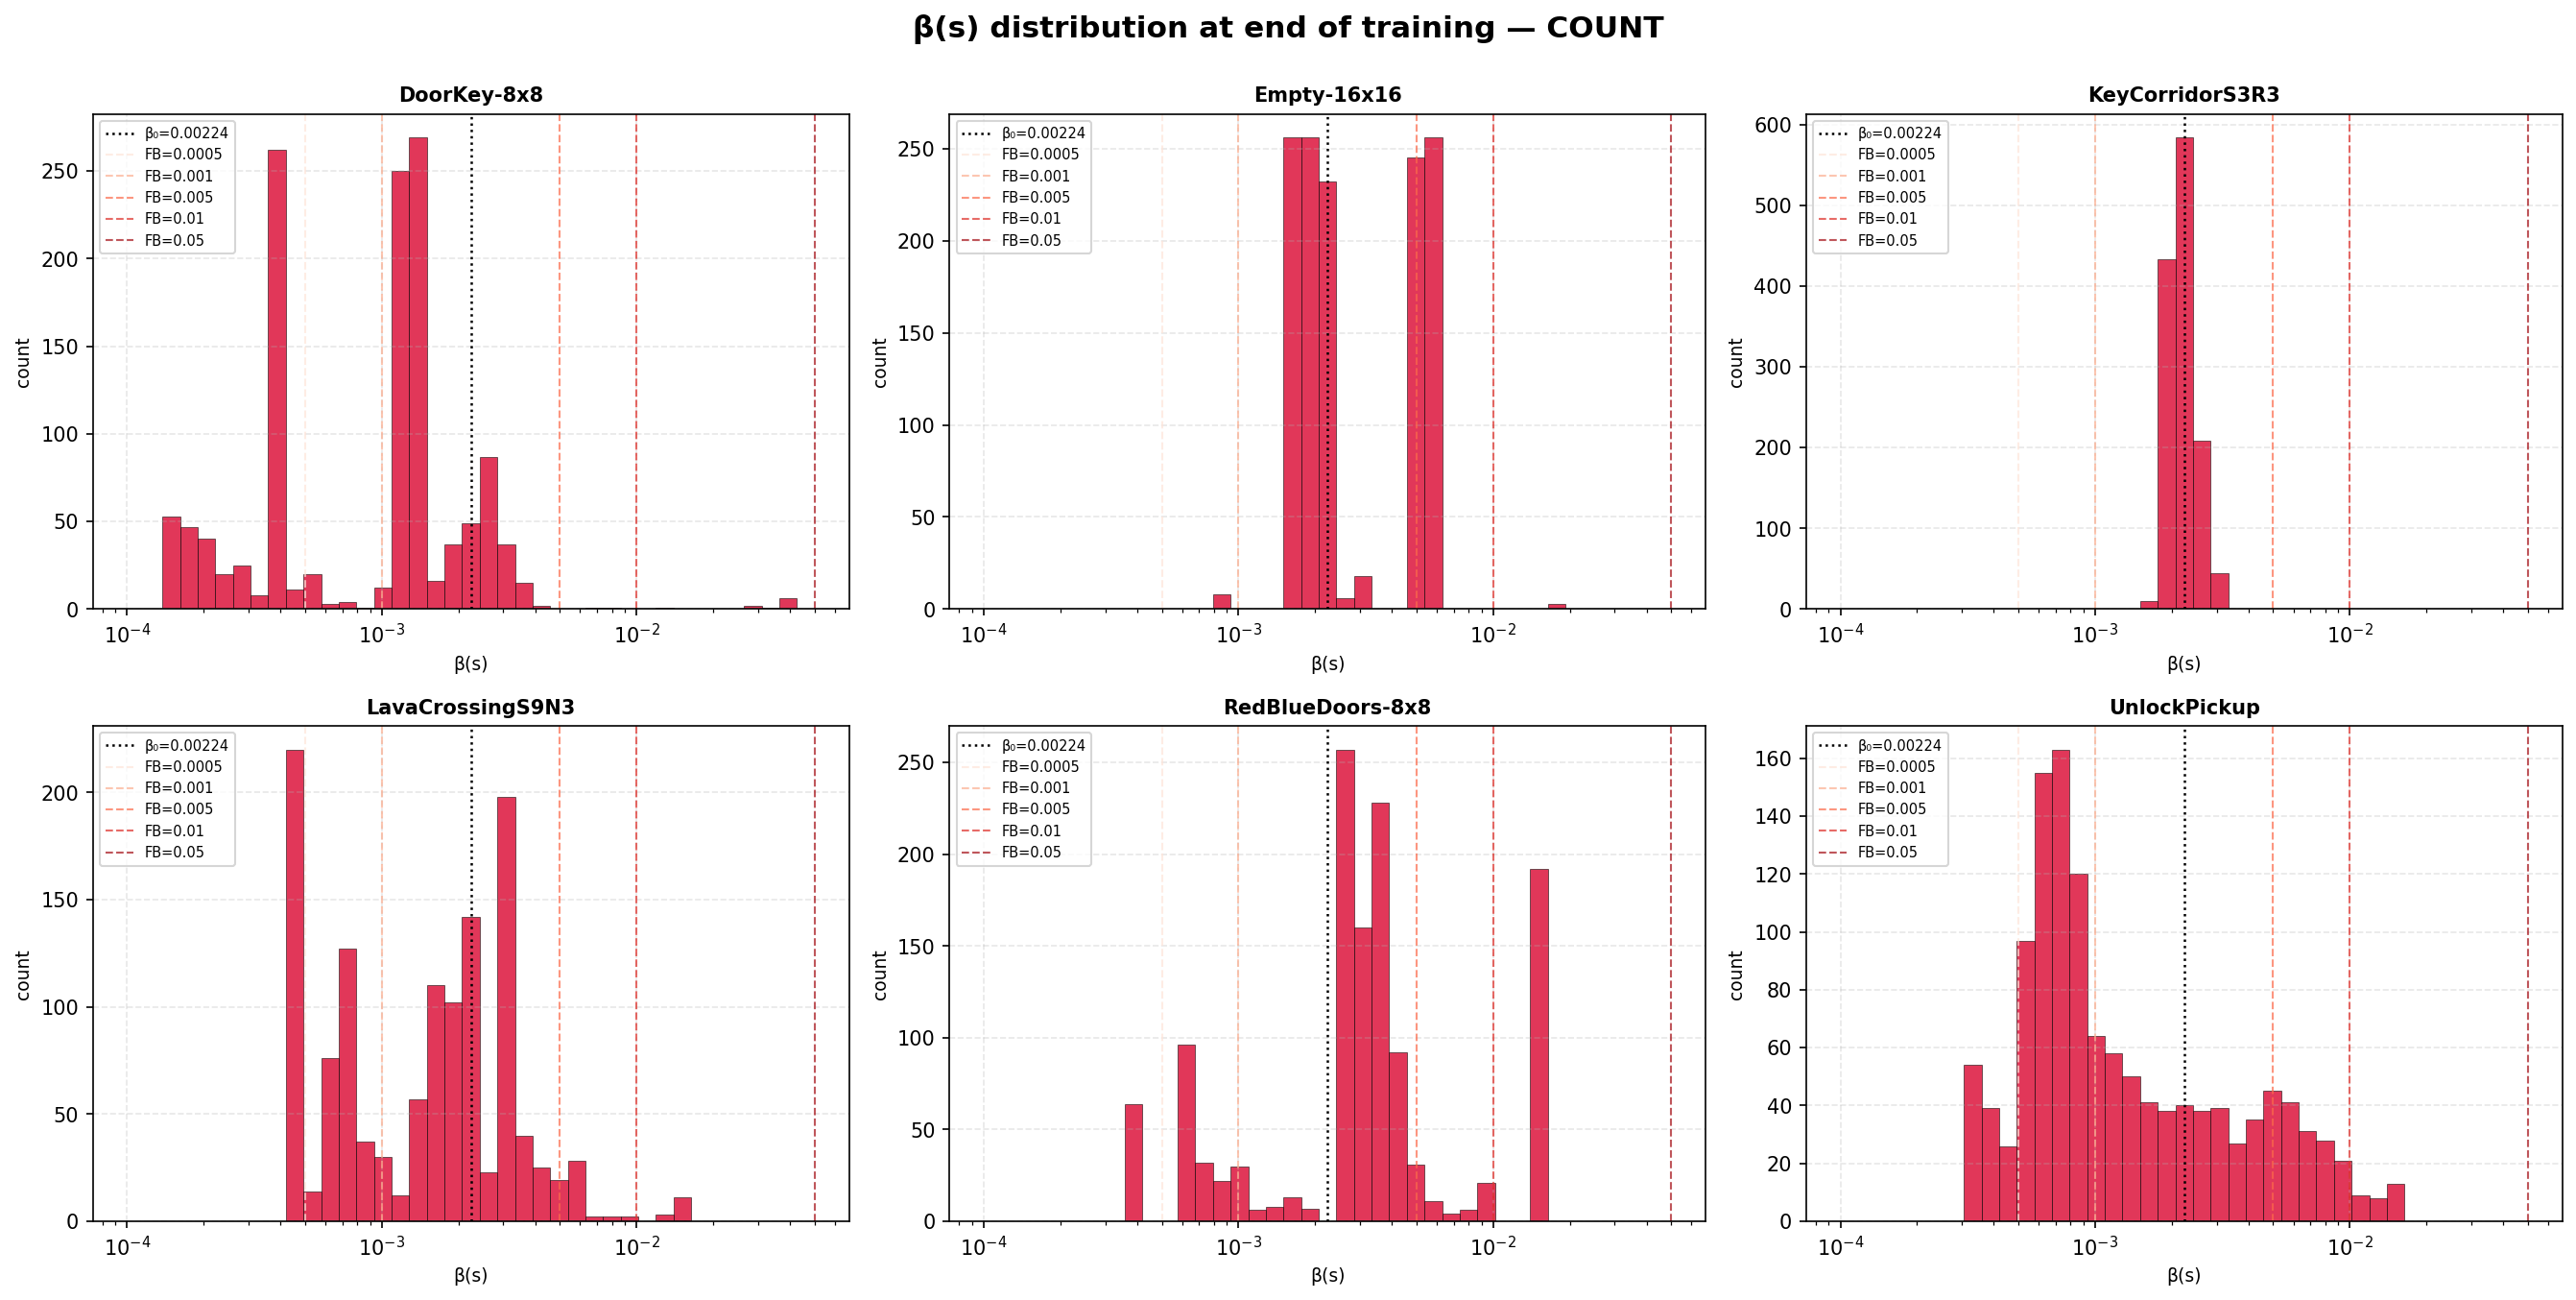
\includegraphics[width=\linewidth]{figures/care_beta_hist_count.png}
\caption{End-of-training distribution of $\beta_\psi(s_t)$ for CARE-COUNT, aggregated across all states sampled during the final $5\%$ of training. Vertical lines mark the geometric-mean prior $\beta_0$ and the five fixed-$\beta$ values used in the baseline sweep.}
\label{fig:care_beta_hist_count}
\end{figure}

\begin{figure}[H]
\centering

\includegraphics[width=\linewidth]{figures/care_beta_hist_icm.png}
\caption{End-of-training distribution of $\beta_\psi(s_t)$ for CARE-ICM. Same conventions as Figure~\ref{fig:care_beta_hist_count}.}
\label{fig:care_beta_hist_icm}
\end{figure}

\begin{figure}[H]
\centering

\includegraphics[width=\linewidth]{figures/care_beta_hist_ride.png}
\caption{End-of-training distribution of $\beta_\psi(s_t)$ for CARE-RIDE. Same conventions as Figure~\ref{fig:care_beta_hist_count}.}
\label{fig:care_beta_hist_ride}
\end{figure}

The end-of-training histograms in Figures~\ref{fig:care_beta_hist_count}--\ref{fig:care_beta_hist_ride} show that the learned $\beta_\psi$ is genuinely state-dependent rather than collapsing to a global value: each module's distribution spans roughly one order of magnitude across visited states, with mass concentrated below $\beta_0$ on environments where the agent has converged. CARE-ICM is the visible exception: its histogram on KeyCorridor (visible in Figure~\ref{fig:care_beta_hist_icm}, lower row) is bimodal with a heavy tail near $\beta_\text{max}$, which matches the failure mode reported in Section~\ref{sec:results_module_level} and is the empirical analogue of the situation described in the second paragraph of Section~\ref{sec:progress_loss}: when the underlying intrinsic signal is large in regions of the state space that are not on the extrinsic-success path, the correlation objective amplifies $\beta_\psi$ in those regions and the policy fails to commit.

The performance profiles in Figures~\ref{fig:profile_count}, \ref{fig:profile_icm}, and \ref{fig:profile_ride} provide a per-module robust comparison: each curve plots the fraction of (environment, seed) pairs whose normalized final reward is at least $\tau$ for $\tau \in [0, 1]$, so a curve that dominates uniformly is preferred under any monotone summary of performance \cite{agarwal2021deep}. CARE-COUNT and CARE-RIDE dominate the fixed-$\beta$ sweep over most of the $\tau$-range; CARE-ICM is dominated by the smallest two fixed-ICM coefficients across most of the range, which is the same conclusion as the per-cell tables but displayed in a way that does not depend on a single threshold.

\begin{figure}[H]
\centering

\includegraphics[width=\linewidth]{figures/profile_count.png}
\caption{Performance profile for the count-based module \cite{agarwal2021deep}: fraction of $(\text{env}, \text{seed})$ pairs whose normalized final reward exceeds threshold $\tau$.}
\label{fig:profile_count}
\end{figure}

\begin{figure}[H]
\centering
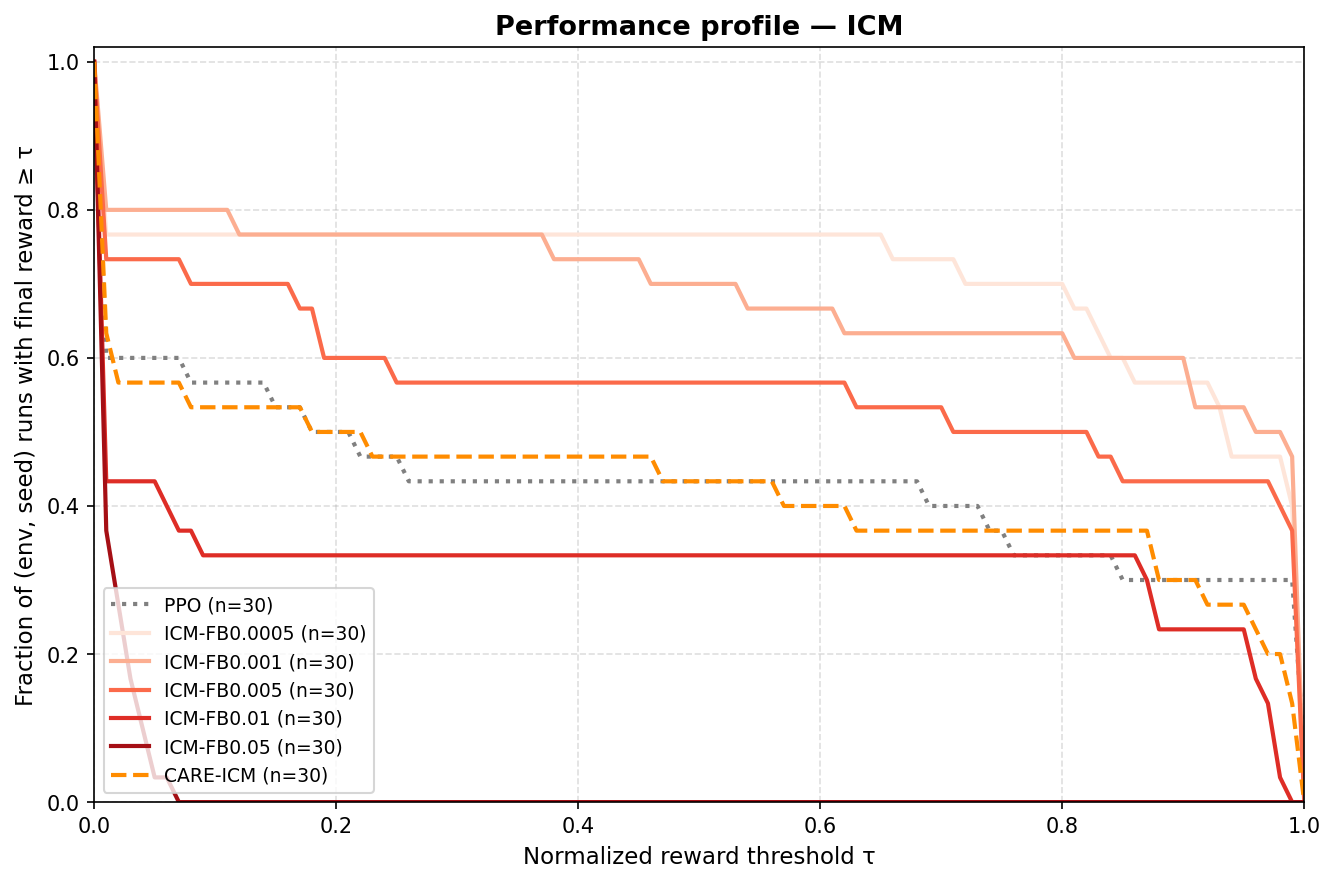
\includegraphics[width=\linewidth]{figures/profile_icm.png}
\caption{Performance profile for the ICM module. Same conventions as Figure~\ref{fig:profile_count}.}
\label{fig:profile_icm}
\end{figure}

\begin{figure}[H]
\centering

\includegraphics[width=\linewidth]{figures/profile_ride.png}
\caption{Performance profile for the RIDE module. Same conventions as Figure~\ref{fig:profile_count}.}
\label{fig:profile_ride}
\end{figure}

\subsection{Discussion}
\label{sec:results_discussion}

The empirical findings can be read against the formal characterization developed in Chapter~\ref{ch:methodology} in three ways.

First, the cold-start regime characterized by Corollary~\ref{cor:degeneration}(i) is observed in practice. On the three environments where extrinsic reward only appears mid-training (KeyCorridor, RedBlueDoors, UnlockPickup), the mean $\beta_\psi$ stays close to the prior $\beta_0$ during the early phase, and the correlation gradient only takes over once the extrinsic advantage acquires a non-degenerate magnitude. This validates the design choice of placing the regularizer's reference value at the geometric mean of the bounds: doing so anchors the cold-start behavior at a value that is neither aggressively exploratory nor effectively zero, and lets the correlation objective drive $\beta_\psi$ in either direction once it has signal to work with.

Second, the gradient direction characterized by Proposition~\ref{prop:gradient_direction} translates into the observed module-by-module pattern. On modules where the intrinsic signal $I^{+,m}$ tends to align with the future extrinsic advantage at the state level --- count-based, where unvisited states sit on the path to the goal, and RIDE, where high-impact transitions sit at the task-relevant decision points --- the within-batch covariance is positive on average and CARE amplifies $\beta_\psi$ at exactly the states where amplification is helpful. On ICM, where the intrinsic signal is driven by forward-model inaccuracy that does not necessarily align with the extrinsic-success path, the conditional covariance is positive in regions that are not goal-directed, and the same gradient amplifies $\beta_\psi$ where amplification harms the policy. The KeyCorridor failure of CARE-ICM is the cleanest empirical instance of this misalignment.

Third, in light of the literature reviewed in Chapter~\ref{ch:literature}, the comparison can be read as a partial answer to the module-agnosticism question raised by Andres et al.\ \cite{andres2025impact}. On the modules whose raw signal already correlates with extrinsic advantage at the state level, CARE matches or exceeds the post-hoc-best fixed coefficient without any environment-specific search; on modules whose raw signal does not, CARE inherits the misalignment and can amplify it. This is consistent with CARE not being a substitute for a well-chosen intrinsic generator but a state-dependent multiplier on top of one --- a multiplier that, by the nature of the correlation objective, can only be as informative as the underlying signal's correlation with extrinsic learning slack. The practical implication is that CARE is a safe default when paired with count-based or impact-driven bonuses on sparse-reward gridworld tasks, and a method to use cautiously when paired with curiosity-by-prediction-error bonuses such as ICM in the same regime.

The principal limitation of the present study is the gridworld scope. MiniGrid environments share a discrete action space, low-dimensional observations, and a reward structure in which extrinsic feedback eventually appears within the $10^6$-step budget. The cold-start regime would be expected to dominate longer in higher-dimensional or richer-observation environments, and the correlation objective would have to remain well-conditioned for considerably more updates before extrinsic signal arrives. Whether the qualitative picture obtained here --- CARE most useful with count-based and impact-driven generators, least useful with prediction-error ones --- transfers to those settings is the natural follow-up direction.
